\section{Introduction}

In this report, I describe an online webapp called \myReportTitle{}, which
collects and displays microclimate data from an \emph{Internet of things} (IoT)
weather station network that I designed and built.The webapp can present live,
historical and forecasted weather data to the user. The live and historical data
is retrieved from a postgreSQL database that collects and stores readings from
my weather station sensor nodes every minute. The historical readings were used
to build a machine learning model that can predict future microclimate specific
weather based on the general forecast.

The weather station network was built using off-the-shelf components and housed
in hand made enclosures. The deployed system consists of four components: two
field sensor nodes capable of reading weather data and transmitting it using a
modern radio protocol called LoRa; a repeater that boosts received LoRa signals;
and an internet connected gateway that uploads the weather data to an online
database. The hardware in this project was tested in a private garden with
deployment to Small Brook Farm in Exeter planned in future. Due to the timeframe
this was not possible within the submission deadline.

\subsection{Motivation and aims}

Weather forecasts are typically based on data from distant weather stations and
large scale models which fail to capture variations that exist within a farm or
even a single field. These local variations, known as microclimates, can differ
significantly even across relatively short distances due to differences in
factors such as elevation, tree cover, or soil type.

For example, in a set of interviews with the owners of Small Brook Farm
(Appendix ~\ref{sec:small-brook-interview}) the owners note that the use of
traditional forecasts for their orchard is not particularly useful for them as
weather forecasts tend to cover wide areas and are not always indicative of very
local conditions. The owners mentioned that the weather conditions across a
single field of apple trees was different, with higher winds on one side
compared to other.

This uncertainty regarding weather conditions has real world consequences for
farmers. For instance, at Small Brook Farm wind speed is a key determinant of
when the farmers can spray their crops with pesticides. Equally, general
forecasts are do not provide accurate enough information to enable farmers to
predict a spring frost that damages crops or to assess the likely incubation
period of pests and diseases.

Agriscanner aims to address this need for accessible local weather forecasting
by giving farmers a weather station platform that can both relay current weather
information from different sections of their field and predict future weather
for their specific location.

\subsection{Contributions}

The key contributions of this paper are:

\begin{itemize}
    \item The development of a low cost, long-range remote weather station
          system with superior range and reduced cost compared to current
          solutions on the market. The long range allows for readings from the
          field to be communicated to the cloud without a need for internet
          access in the field.
    \item A publicly available web application for visualising live data from
          multiple field locations, that demonstrates a high degree of usability
          across both mobile and desktop platforms, as confirmed by quantitative
          System Usability Scale (SUS) evaluation.
    \item A method for enabling microclimate forecasting using a machine
          learning process that compares local sensor data with broader regional
          weather forecasts. This aims to give farmers access to a hyper-local
          forecast of future weather conditions that is specific to their field
          and optimise agricultural tasks such as spraying.
\end{itemize} 

\subsection{Project schematic and layout}

\begin{figure}[H]
    \centering
    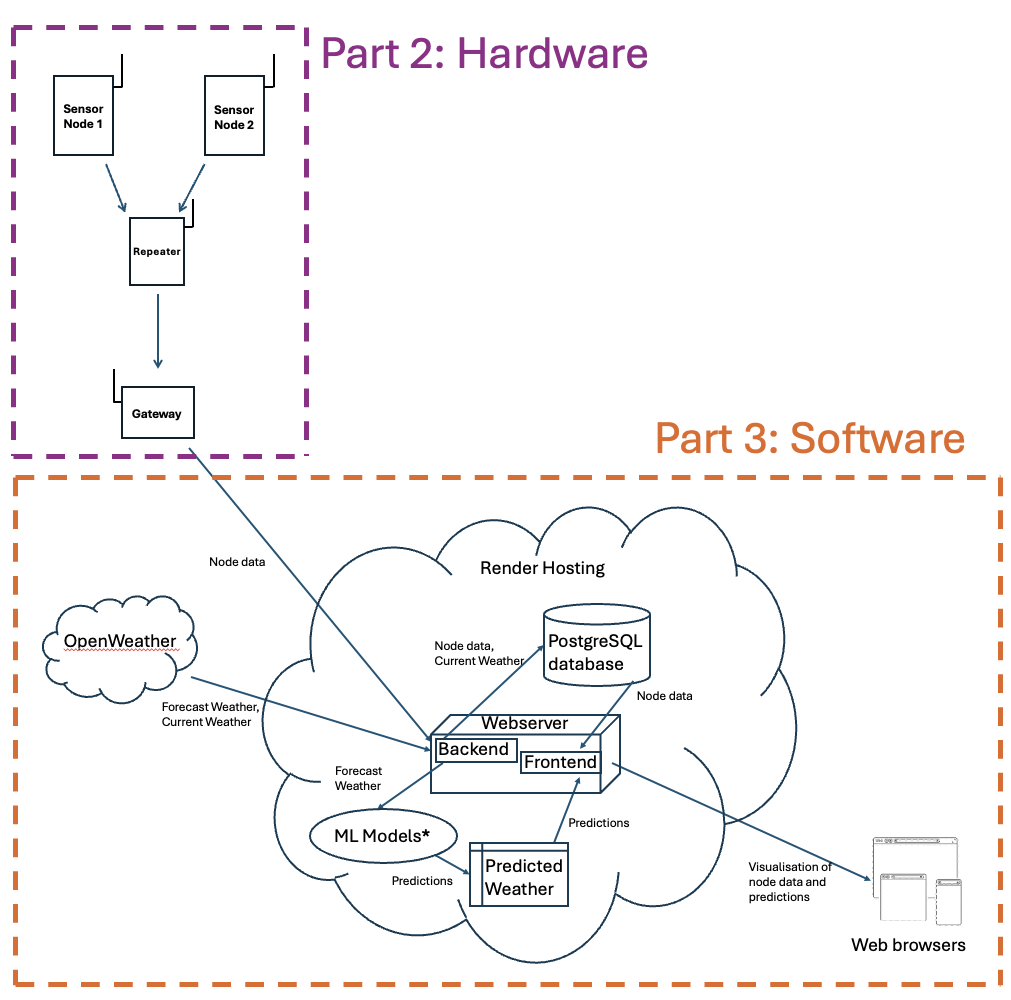
\includegraphics[width=1\textwidth]{contents/part-1/fig1/project-schema.png}
    \par\vspace{1pt} \noindent\begin{minipage}{0.95\textwidth}
        \centering\footnotesize\textsuperscript{*} Training the machine learning
        models is not pictured on this graph.
    \end{minipage}
    \par\vspace{1pt}
    \caption{Schematic of entire project showing data paths}
    \label{fig:project-schema}
\end{figure}

Figure \ref{fig:project-schema} shows the design of the my entire project, which
has been split into hardware and software categories that correspond to parts 2
and 3 of this dissertation.  A zoomed in version of each category is shown on
the overview of its respective part (see hardware overview in Chapter
\ref{sec:hardware-overview} , and software overview in Chapter
\ref{sec:software-overview}).

Part 1 provides the technical background to understand the project, including an
overview of the core technologies used and a review of related work in the
field.

Part 4 then offers a critical evaluation of the system, discussing its
performance, usability, and limitations, as well as highlighting opportunities
for future development improvements and research.